\chapter{Detalle de CDF para bytes por vértice en estructuras compactas, para cada función de ranking}
\label{anexo:cdf}

\centering
\textbf{Anexo \thechapter:  1 de 4}
\begin{minipage}{1\textwidth}
    \centering
    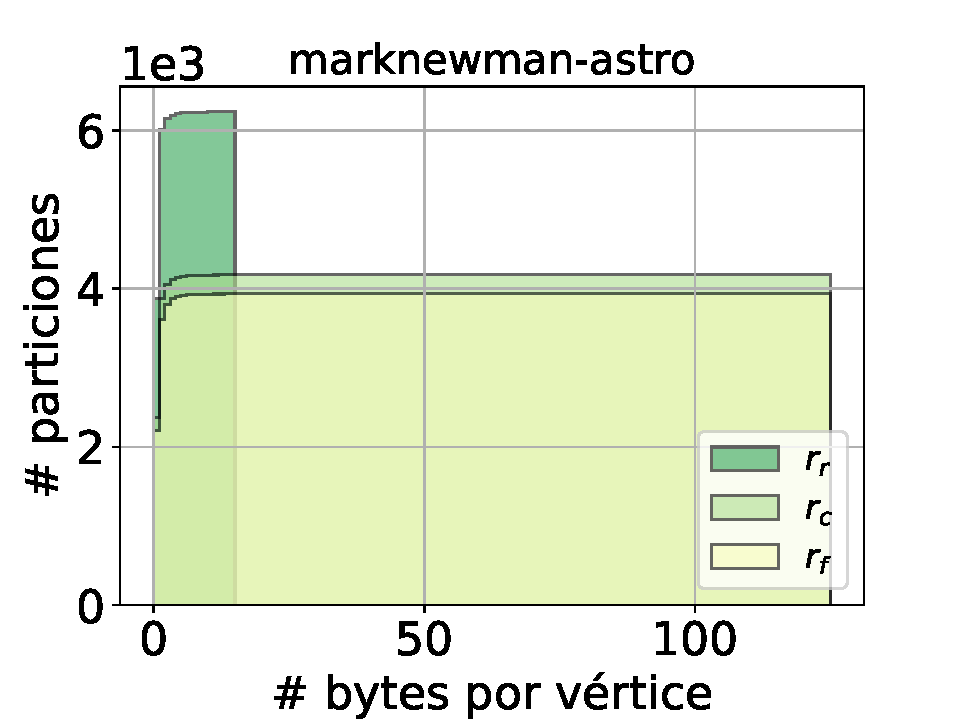
\includegraphics[width=.9\linewidth]{img/cdf/marknewman-astro.pdf} \\
    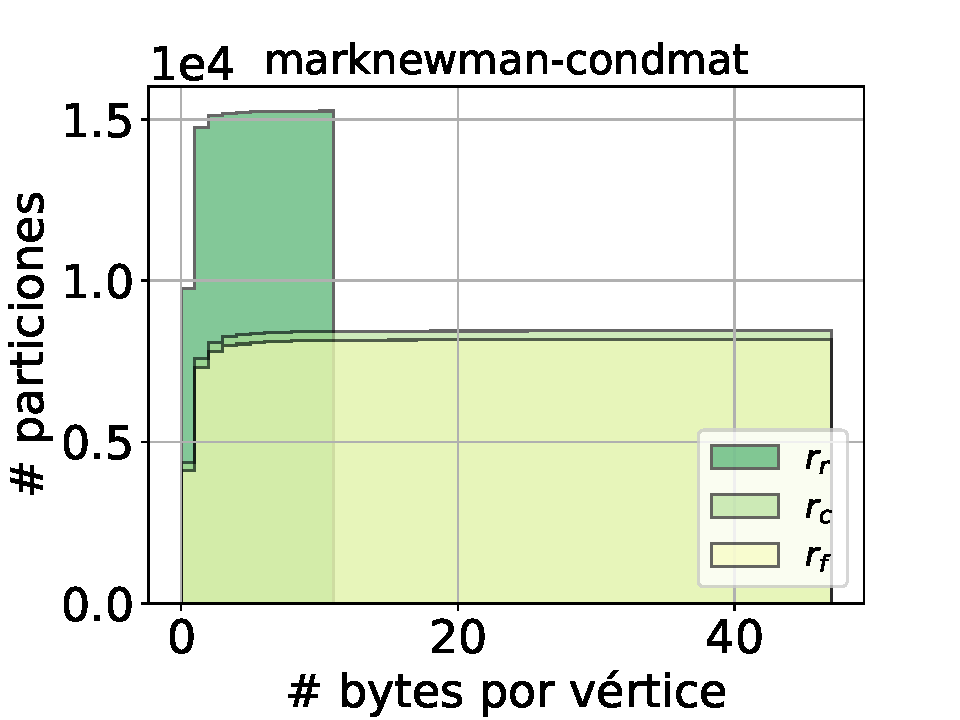
\includegraphics[width=.9\linewidth]{img/cdf/marknewman-condmat.pdf} \\		
\end{minipage}

\centering
\begin{minipage}{1\textwidth}
    \centering
	\textbf{Anexo \thechapter:  2 de 4}
    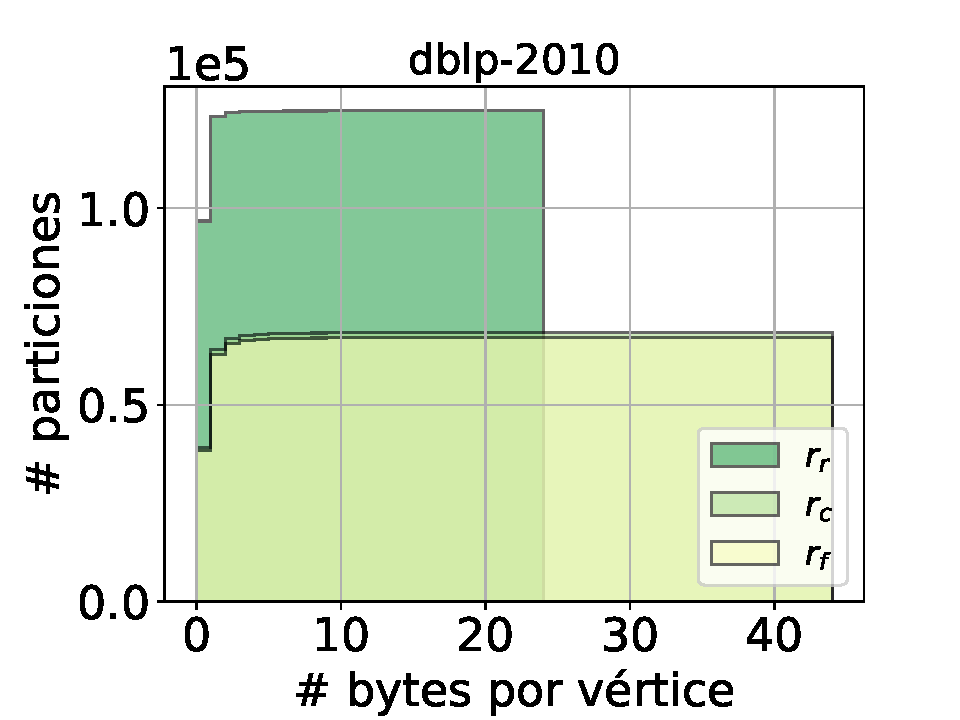
\includegraphics[width=.9\linewidth]{img/cdf/dblp-2010.pdf} \\
    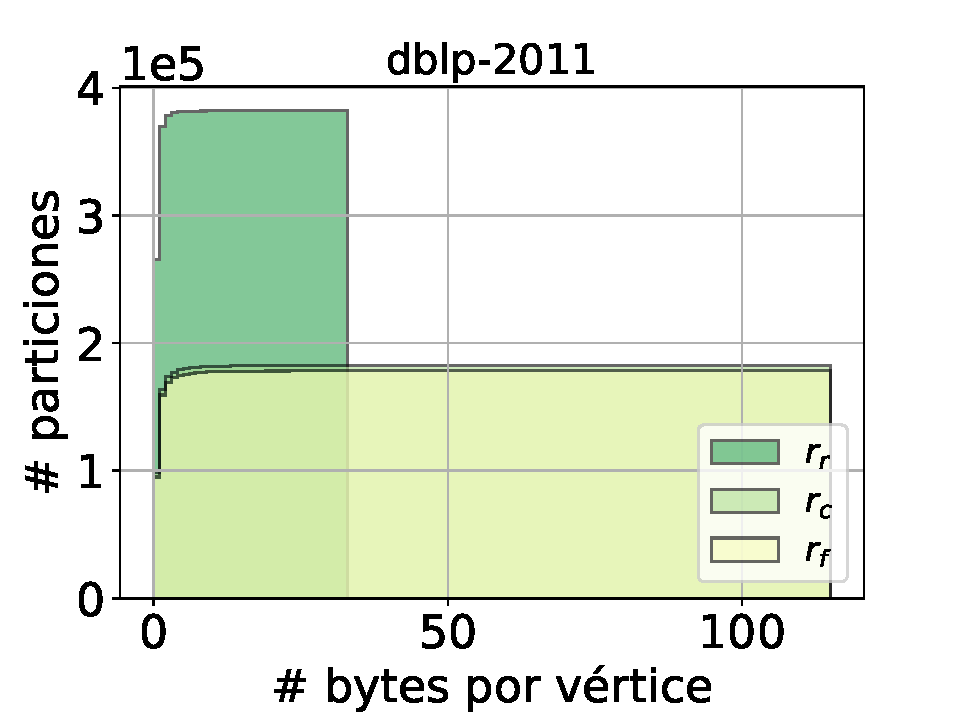
\includegraphics[width=.9\linewidth]{img/cdf/dblp-2011.pdf} \\
\end{minipage}

\centering
\begin{minipage}{1\textwidth}
    \centering
    \textbf{Anexo \thechapter:  3 de 4}
    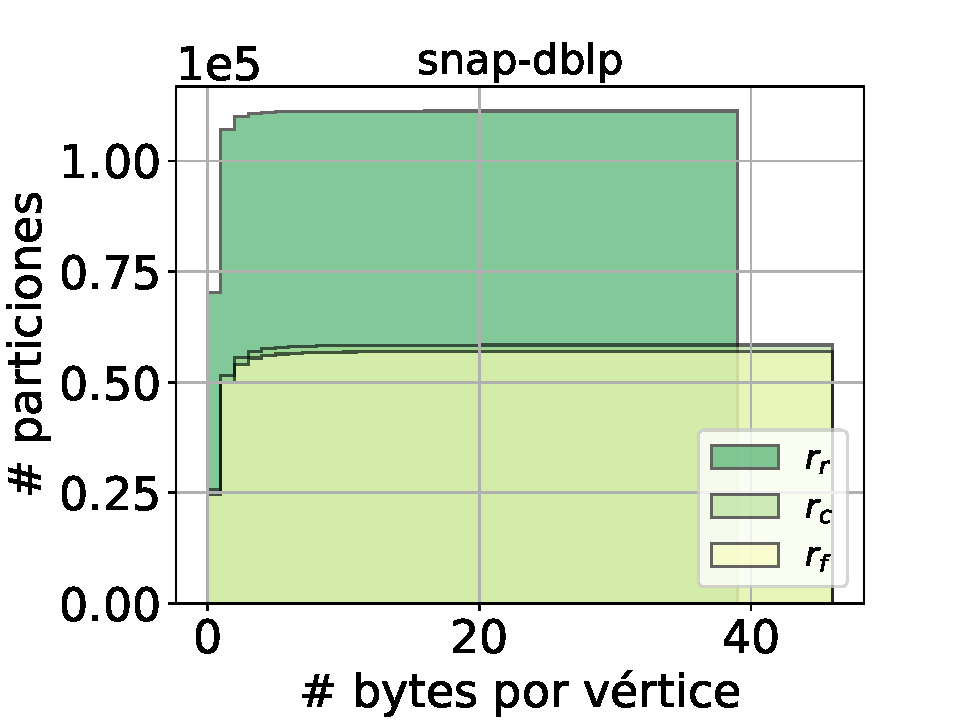
\includegraphics[width=.9\linewidth]{img/cdf/snap-dblp.pdf} \\
    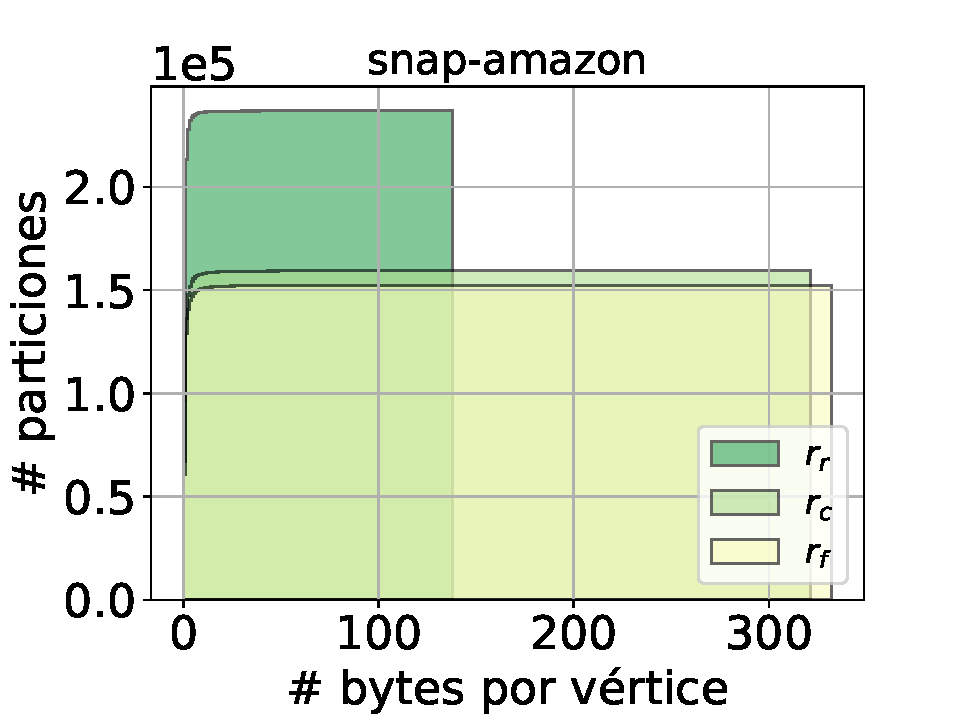
\includegraphics[width=.9\linewidth]{img/cdf/snap-amazon.pdf} \\
\end{minipage}

\centering
\begin{minipage}{1\textwidth}
    \centering
    \textbf{Anexo \thechapter:  4 de 4}
    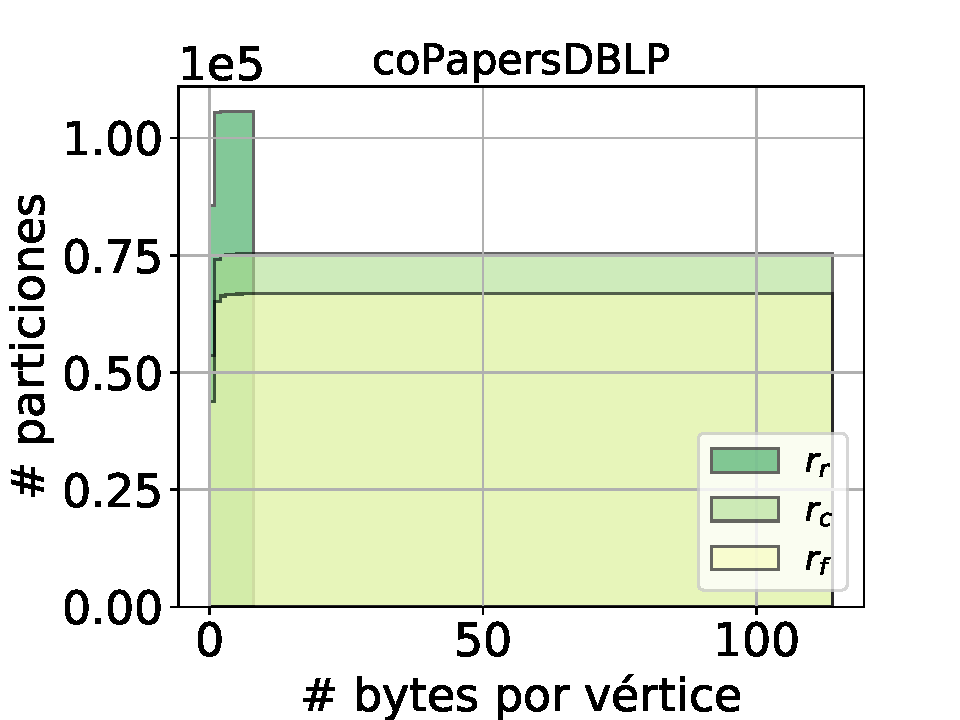
\includegraphics[width=.9\linewidth]{img/cdf/coPapersDBLP.pdf} \\
    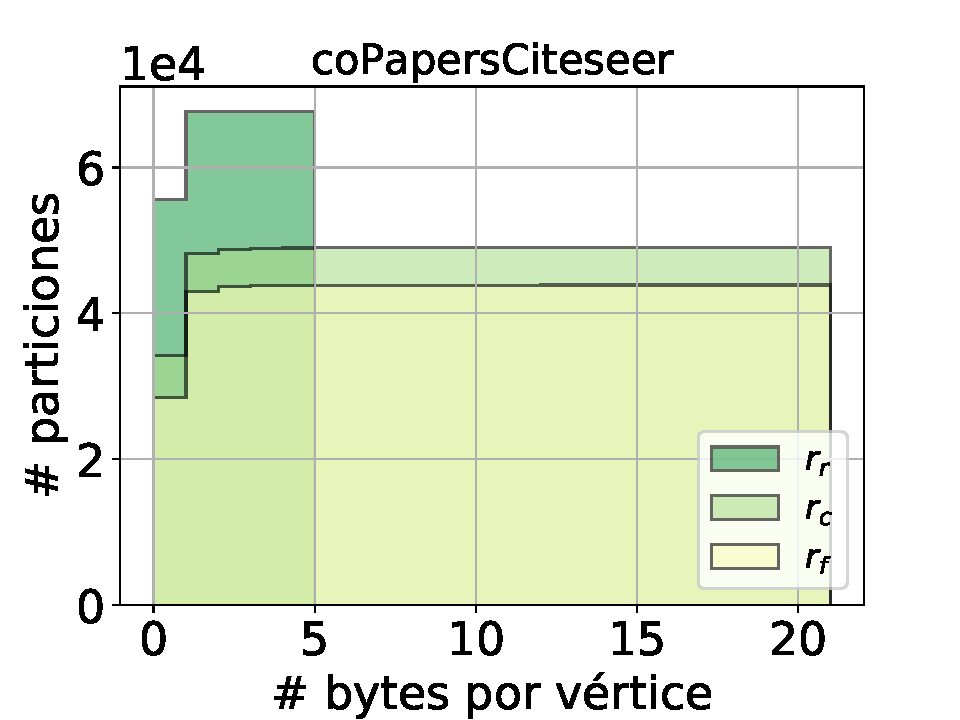
\includegraphics[width=.9\linewidth]{img/cdf/coPapersCiteseer.pdf} \\
\end{minipage}
